\section{Design}
\label{sec:design}

Tejo comprises three components, namely a set of fault injection tools, a data handler, and a learning model. These components interoperate into two distinct phases: learning and detection phase. While the first phase allows us to evaluate the performance of a NewSQL database under anomalies, the second permits the detection of these anomalies. Figure~\ref{fig:tejo_overview} depicts the components and the two-phase functioning of Tejo.


\begin{figure*}
        \centering
        \begin{subfigure}[b]{0.48\textwidth}
               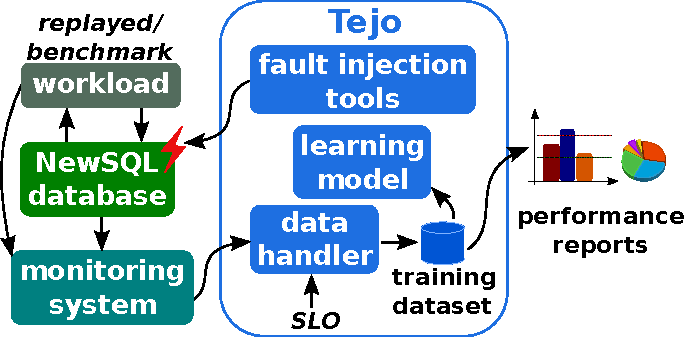
\includegraphics[width=1\textwidth]{inputs/img/tejo_overview_learning_newsql}
                \caption{Learning phase.}
                \label{fig:tejo_overview_learning}
        \end{subfigure}
	\rulesep
        \begin{subfigure}[b]{0.48\textwidth}
                  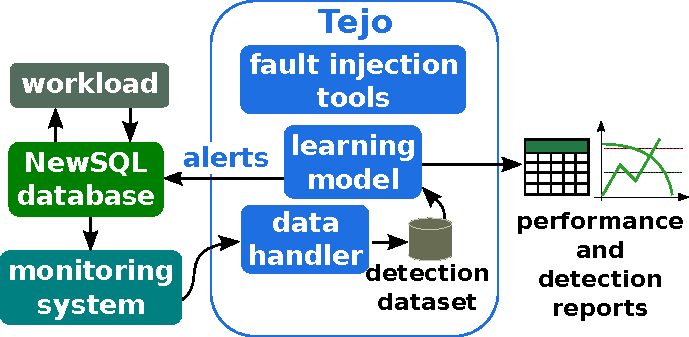
\includegraphics[width=1\textwidth]{inputs/img/tejo_overview_detection_newsql}
                \caption{Detection phase.}
                \label{fig:tejo_overview_detecting}
        \end{subfigure}
        \caption{Tejo operates in two distinct phases: learning and detection phase.}\label{fig:tejo_overview}
\end{figure*}

\subsection{The components of Tejo}
\label{subsec:tejo_components}

\subsubsection{Fault injection tools.} 
To provoke performance anomalies, this component emulates four categories of faulty events in VMs of a NewSQL database cluster. 

\emph{Network faults}. Communication issues are common in distributed systems. To analyse their impact, we inject three types of network faults, namely packet loss, network latency, and limping network. Packet loss and network latency emulates interconnection issues, such as network partition. Limping network reproduces anomalies previously observed by Do \emph{et al.}~\cite{do2013limplock}, where the transmission rate of limping network interface is smaller than the manufacturer's specification. 

\emph{Memory faults}. As NewSQL databases fit the entire data to the main memory, they become more vulnerable to anomalies in memory availability. To provoke such anomalies, we make arbitrary amounts of main memory unavailable. As a result, the database instance is likely to perform more costly disk I/O operations. A typical example of this fault is a VM running out of memory due to a misconfiguration, memory leaking, overloading, or an unbalanced resource allocation.

\emph{Disk faults}. Although most NewSQL databases manage data in main memory, disk-intensive processes may have an impact of its performance. This category of fault emulates an arbitrary number of jobs performing several disk operations, including writes, reads, and file syncs.  

\emph{CPU faults}. CPU is a key resource in a virtual machine. As unattended number of processes compete the database instance to CPU resources, they may undermine the performance of the database cluster. The CPU fault emulates an arbitrary number of jobs performing arithmetic operations to overload the VM cores. 


\subsubsection{The data handler.} 
This component computes data from the monitoring system (i) to collect the performance counters of a NewSQL database and (ii) to provide data to characterize performance anomalies.

\emph{Collect the performance counters of a NewSQL database}. The data handler samples monitoring data to collect the current state of the NewSQL cluster, as depicted in Figure~\ref{fig:tejo_overview}. To this end, it frequently communicates with the monitoring system to fetch raw monitoring data and to convert it into useful, aggregated information. The content of the resulting aggregated information depends on the aim of each functioning phase, learning or detection, detailed below. 

\emph{Providing data to characterize performance anomalies}. After aggregating samples of monitoring data, the data handler organizes this data into \emph{feature vectors}. These vectors represent the state of the VMs of the database cluster or the workload. The vectors are stored in datasets for performance analysis or anomaly detection. 

\subsubsection{The learning model.} 
The learning model is at the heart of the Tejo scheme. The purpose of this model, the so-called predictive task, is to characterize the behaviour of VMs under performance anomalies. Given an i.i.d. sample $(\inpseq,\rel)$, described in Subsection~\ref{sec:background}, we model our predictive task as a classification problem, whose inputs and outputs are defined as follows.

\emph{Inputs}. We represent the input space $\inpseq$ as a VM running a database instance. This input data corresponds to a feature vector computed by the data handler component. The size of the feature vector matters. In general, the higher the dimension of this vector, the higher the predictive efficiency is. However, an increase in the input dimension rises the computational cost of predictions.

\emph{Outputs}. The supervision $\rel$ associated to each input VM $\inpseq$ is based on five possible classes, $\mathcal{Y} \in \{0,1,2,3,4\}$, whose labels are \emph{normal}, \emph{network-related anomaly}, \emph{memory-related anomaly}, \emph{disk-related anomaly}, and \emph{CPU-related anomaly} respectively. Depending on the phase of Tejo (detailed below), these labels are assigned by either computing the training dataset or by a learning algorithm.

\subsection{Two-phase functioning}
\label{subsec:tejo_phases}

\subsubsection{Learning phase.} In this phase, Tejo learns the behaviour of the database cluster under anomalies and reports on its performance.

\emph{Requirements}. As illustrated in Figure~\ref{fig:tejo_overview_learning}, Tejo relies on an already existing monitoring system to poll performance counters from both VMs and workload. To measure the cluster-wide performance counters, we assume that the workload can be replayed or run through a benchmark tool. We consider that Tejo's analyst specifies expected SLO metrics, such as average throughput and $99^{th}$ percentile latency. The analyst must also specify parameters of the fault campaign and running experiments, including intensity and duration of each fault, number of injections, and interval between consecutive fault injections. 

\emph{Functioning.} As the replayed/benchmark workload runs, the fault injection tool performs a fault injection campaign to emulate performance anomalies. Meanwhile, performance counters from both the workload and VMs running the database cluster are collected by the monitoring system and computed by the data handler component. As the data handler computes the monitoring data in feature vectors, it adds information about injected faults and labels. Labels correspond to output classes of learning model and are added with respect to SLO metrics. The feature vectors are then stored in the training dataset. After running the workload and accomplishing the fault injection campaign, the learning model computes the feature vectors of VMs from the training dataset.

\emph{Reports.} Besides providing data to learn the behaviour of anomalous VMs, analysts can observe the impact of anomalies in the throughput and $99^{th}$ percentile latency. They may evaluate which anomalies cause SLO  violations, gaining more insight into the efficiency of existing fault-tolerance mechanisms. 

\subsubsection{Detection phase.} In this phase, Tejo reports on the efficiency of the learning model and performs anomaly detection in VMs at runtime. 

\emph{Requirements}. Similar to the training phase, Tejo relies on an existing monitoring platform to gather data for predictions. It requires that the learning model has already been trained as detailed in learning phase described above. We assume that SLO targets and the workload are the same as those of the learning phase. 

\emph{Functioning.} While the NewSQL database serves the workload, the data handler gathers the monitoring data and creates feature vectors of VMs in the detection dataset. As soon as a new feature vector is created, the learning model computes it to detect performance anomalies whenever they occur.  

\emph{Reports.} Tejo's learning model predicts labels of incoming feature vectors. Then alerts are generated about detected anomalies. These alerts may be handled by the database to trigger recovery procedures. Besides generating alerts, it reports on the efficiency of the learning model, including comparing different learning algorithms, ranking performance counters with regard to their importance, calculating the computational cost, and verifying model over-fitting  or under-fitting. 

